\input ../SlidePreamble
\input ../preamble

\begin{document}

{\Huge

  \centerline{\bf TTIC 31230, Fundamentals of Deep Learning}
  \bigskip
  \centerline{David McAllester, Winter 2019}
  \vfill
  \vfill
  \centerline{\bf Deep Graphical Models}
\vfill
\vfill
\vfill

\slide{Distributions on Exponentially Large Sets}

\vfill
{\color{red}
$$\Phi^* = \argmin_\Phi E_{(x,y) \sim \mathrm{Pop}}\;-\ln \;P(y|x)$$

\vfill
$$\Phi^* = \argmin_\Phi E_{y \sim \mathrm{Pop}}\;-\ln \;P(y)$$
}

{\color{red} The structured case:} $y \in {\cal Y}$ where ${\cal Y}$ is discrete but {\color{red} iteration over $\hat{y} \in {\cal Y}$ is infeasible}.
\slide{Semantic Segmentation}
\centerline{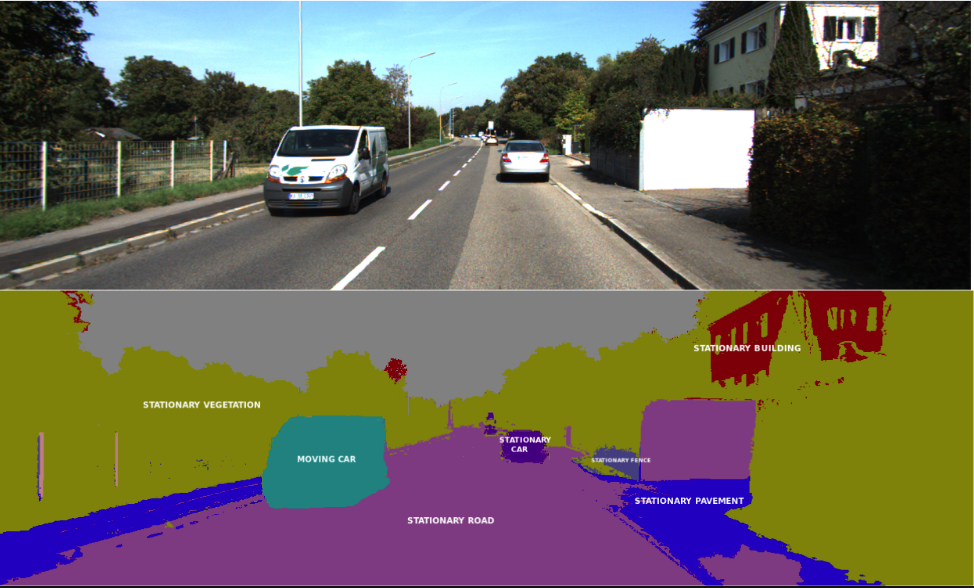
\includegraphics[height = 2.5in]{../images/SemSeg}}

\vfill
We want to assign each pixel to one of $C$ semantic classes.

\vfill
For example ``person'', ``car'', ``building'', ``sky'' or ``other''.

\slide{Constructing a Graph}

We construct a graph whose nodes are the pixels and where there is an edges between each pixel and its four nearest neighboring pixels.

\vfill
$$\begin{array}{ccccc}
 & & {\color{red} j(i,\mathrm{up})} \\
 & & | \\
 {\color{red} j(i,\mathrm{right})}\;\;\;\; & -& i & -& \;\;\;\;{\color{red} j(i,\mathrm{left})} \\
 & & | \\
 & & {\color{red} j(i,\mathrm{down})}
 \end{array}$$

\slide{Labeling the Nodes of the Graph }


$\hat{y} $ assigns a semantic class $\hat{y}[i]$ to each node (pixel) $i$.

\vfill
We assign a score to $\hat{y}$ by assigning a score to each node and each edge of the graph.

{\color{red} $$s(\hat{y}) = \sum_{i \in \mathrm{Nodes}}\; s_n[i,\hat{y}[i]]\; + \sum_{i \in \mathrm{Nodes},\;d \in \{L,R,U,D\}}\;s_e[i,d,\hat{y}[i],\;\hat{y}[j(i,d)]]$$}
\centerline{Node Scores \hspace{6em}Edge Scores \hspace{3em}~}


\slide{Computing the Node and Edge Scores}

We assume a CNN computing {\color{red} node and edge score tensors}
\vfill
$$\begin{array}{lrcl}
& \mbox{intput image} \\
& \vdots \\
& \mbox{CNN} \\
& \vdots \\
\mathrm{for}\;i,c & \;{\color{red} s_n[i,c]} & = & \ldots \\
\mathrm{for}\;i,d,c,c' & {\color{red} s_e[i,d,c,c']} & = & \ldots \\
\end{array}$$

\vfill
The tensor {\color{red} $s_n[i,c]$} holds $PC$ scores.

\vfill
The tensor {\color{red} $s_e[i,d,c,c']$} holds $4PC^2$ scores.

\slide{Computationally Infeasible Exponential Softmax}
$$\begin{array}{lrcl}
& \mbox{intput image} \\
& \vdots \\
& \mbox{CNN} \\
& \vdots \\
\mathrm{for}\;i,c & \;{\color{red} s_n[i,c]} & = & \ldots \\
\mathrm{for}\;i,d,c,c' & {\color{red} s_e[i,d,c,c']} & = & \ldots
\end{array}$$

\vfill
$$\begin{array}{lrcl}
\mbox{for}\;\hat{y} & {\color{red} s(\hat{y})} & = & \sum_i\;s_n[i,\hat{y}[i]] + \sum_{i,d}\;s_e[i,d,\hat{y}[i],\;\hat{y}[j[i,d)]] \\
\mbox{for}\;\hat{y} & {\color{red} P(\hat{y})} & = & \expsoftmax_{\hat{y}}\;s(\hat{y}) \;\;\mbox{\color{red} all possible $\hat{y}$} \\
 & {\cal L} & = & {\color{red} - \ln P(y) \;\;\;\mbox{gold label $y$}}
\end{array}$$

\slide{Exponential Softmax is Typically Intractable}
\centerline{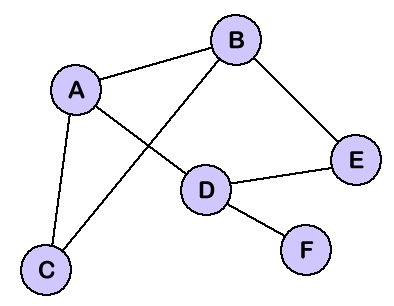
\includegraphics[height= 1.5in]{../images/Graph}}
\medskip
$\hat{y} $ assigns a label $\hat{y}[i]$ to each node $i$.

\vfill
$s(\hat{y})$ is defined by a sum over node and edge tensor scores.

\vfill
$P(\hat{y})$ is defined by an exponential softmax over $s(\hat{y})$.

\vfill
Computing $Z$ in general is \#P hard.

\slide{Back-Propagation Through Intractable Softmax}

$$\begin{array}{lrcl}
& \vdots \\
\mathrm{for}\;i,c & \;{\color{red} s_n[i,c]} & = & \ldots \\
\mathrm{for}\;i,d,c,c' & {\color{red} s_e[i,d,c,c']} & = & \ldots
\end{array}$$

$$\begin{array}{lrcl}
\mbox{for}\;\hat{y} & {\color{red} s(\hat{y})} & = & \sum_i\;s_n[i,\hat{y}[i]] + \sum_{i,d}\;s_e[i,d,\hat{y}[i],\;\hat{y}[j[i,d)]] \\
\mbox{for}\;\hat{y} & {\color{red} P(\hat{y})} & = & \expsoftmax_{\hat{y}}\;s(\hat{y}) \;\;\mbox{\color{red} all possible $\hat{y}$} \\
 & {\cal L} & = & {\color{red} - \ln P(y) \;\;\;\mbox{gold label $y$}}
\end{array}$$

\vfill
We need to compute {\color{red} $s_n.\grad[i,c]$} and {\color{red} $s_e.\grad[i,d,c,c']$}.

\vfill
Although exact calculation is intractable, in practice the gradients can be approximated.

\slide{Model Marginals Theorem}

Theorem:
\begin{eqnarray*}
    s_n.\mathrm{grad}[i,c] & = &  {\color{red} P_{\hat{y} \sim P_s}(\;\;\hat{y}[i] = c\;\;)} \\
    & & \;\;\;\;\;- \bbone[\;\;y[i] = c\;\;] \\
    \\
    s_e.\mathrm{grad}[i,d,c,c'] & = &  {\color{red} P_{\hat{y} \sim P_s}(\;\;\hat{y}[i] = c \; \wedge \; \hat{y}[j(i,d)] = c'\;\;)} \\
    & & \;\;\;\;\;- \bbone[\;\;y[i] = c\; \wedge \; y[j(i,d)] =
    c'\;\;]
\end{eqnarray*}

\vfill
To approximately back-propagate log loss of an intractable graphical model it suffices to approximate
{\color{red} the model marginals} in red above.

\slide{Proof of Model Marginals Theorem}

We consider the case of node marginals.

{\huge \begin{eqnarray*}
    s_n.\mathrm{grad}[i,c] & = & \partial (\ln Z - s(y))\;/\;\partial s_n[i,c] \\
    & = & \left(\frac{1}{Z} \sum_{\hat{y}} e^{s(\hat{y})} \left(\partial s(\hat{y})/\partial s_n[i,c]\right)\right)
    - \left(\partial s(y) /\partial s_b[i,c]\right)    \\
    \\
    & = & \left(\sum_{\hat{y}} P_s(\hat{y}) \left(\partial s(\hat{y})/\partial s_n[i,c]\right)\right)
    - \left(\partial s(y) /\partial s_n[i,c]\right)    \\
    \\
    & = & E_{\hat{y} \sim P_s}\bbone[\hat{y}[i] = c]
    - \mathbbm{1}[y[i] = c] \\
    \\
    & = & {\color{red} P_{\hat{y} \sim P_s}(\hat{y}[i] = c)}
      - \mathbbm{1}[y[i] = c]
\end{eqnarray*}
}

\slide{Methods of Approximating Model Marginals}

MCMC Sampling

\vfill
Pseudolikelihood

\vfill
Contrastive Divergence

\vfill
Loopy Belief Propagation (loopy BP)

\slide{MCMC Sampling}
The model marginals, such as the node marginals
 ${\color{red} P_s(\hat{y}[i]=c)}$, can be estimated by sampling $\hat{y}$ from $P_s(\hat{y})$.

\vfill
We will design a Markov process whose states are segmentations $\hat{y}$ and whose stationary distribution is $P_s$.

\vfill
We will run the process past its mixing time to get a sample $\hat{y}$ from $P_s$.

\slide{A Neighbor Relation on States}

We will say that segmentations (states) $\hat{y}$ and $\hat{y}'$ are neighbors if they differ in exactly one pixel.

\vfill
Note that the number of neighbors of $\hat{y}$ is $P(C-1)$.

\vfill
We will write $N(\hat{y})$ for the set of neighbors of $\hat{y}$.


\vfill
For the correctness of the Metropolis algorithm we need that all states have the same number of neighbors
and $\hat{y}' \in N(\hat{y})$ if and only if $\hat{y} \in N(\hat{y}')$.

\slide{The Metropolis Markov Chain}

We need to define state transition probabilities.

\vfill
In the {\color{red} Metropolis algorithm} we do the following.

\vfill
\vfill
Pick an initial state $\hat{y}$ and then repeat:
\vspace{-2ex}
\begin{quotation}
\noindent \begin{enumerate}
        \item Pick a neighbor $\hat{y}' \in N(\hat{y})$ uniformly at random.

        \vfill
        \item If $P_s(\hat{y}') \geq P_s(\hat{y})$ then do $\hat{y} = \hat{y}'$

  \vfill
\item If $P_s(\hat{y}') < P_s(\hat{y})$ then do $\hat{y} = \hat{y}'$ with probability $\frac{P_s(\hat{y}')}{P_s(\hat{y})}$
  \end{enumerate}  
\end{quotation}

\slide{The Metropolis Markov Chain}
Pick an initial state $\hat{y}$ and then repeat:
\vspace{-2ex}
\begin{quotation}
\noindent \begin{enumerate}
        \item Pick a neighbor $\hat{y}' \in N(\hat{y})$ uniformly at random.

        \vfill
        \item If $P_s(\hat{y}') \geq P_s(\hat{y})$ then do $\hat{y} = \hat{y}'$

  \vfill
\item If $P_s(\hat{y}') < P_s(\hat{y})$ then do $\hat{y} = \hat{y}'$ with probability $\frac{P_s(\hat{y}')}{P_s(\hat{y})}$
  \end{enumerate}  
\end{quotation}

\vfill
Note that we can determine which probability is larger just by comparing scores --- we do not need to know $Z$.

\vfill
Also note that the ratio $P_s(\hat{y}')/P_s(\hat{y})$ can be computed from the scores without knowledge of $Z$.

\slide{The Metropolis Markov Chain}
We need to show that $P_s$ is a stationary distribution of this process.

\vfill
We must show that if we select $\hat{y}_t$ from $P_s$, and then select $\hat{y}_{t+1}$ using the transition probabilities,
then the distribution on $\hat{y}_{t+1}$ is also $P_s$.

\slide{The Metropolis Markov Chain}

{\huge
\begin{eqnarray*}
P'(\hat{y}) & = & \sum_{\hat{y}'}\;P_s(\hat{y}')P_{\mathrm{Trans}}(\hat{y}\;|\;\hat{y}') \\
\\
& = & P_s(\hat{y})P_{\mathrm{Trans}}(\hat{y}\;|\;\hat{y}) + \sum_{\hat{y}' \in N(\hat{y})}\;P_s(\hat{y}')P_{\mathrm{Trans}}(\hat{y}\;|\;\hat{y}') \\
\\
& = & P_s(\hat{y})\left(1 - \sum_{\hat{y}' \in N(\hat{y})} P_{\mathrm{Trans}}(\hat{y}'\;|\;\hat{y})\right) + \sum_{\hat{y}' \in N(\hat{y})}\;P_s(\hat{y}')P_{\mathrm{Trans}}(\hat{y}\;|\;\hat{y}') \\
\\
\\
& = & P_s(\hat{y}) + \sum_{\hat{y}' \in N(\hat{y})}\;P_s(\hat{y}')P_{\mathrm{Trans}}(\hat{y}\;|\;\hat{y}') - P_s(\hat{y})P_{\mathrm{Trans}}(\hat{y}'\;|\;\hat{y})
\end{eqnarray*}
}

\slide{Detailed Balance}

{\huge
\begin{eqnarray*}
P'(\hat{y}) & = & P_s(\hat{y}) + \sum_{\hat{y}' \in N(\hat{y})}\;{\color{red} P_s(\hat{y}')P_{\mathrm{Trans}}(\hat{y}\;|\;\hat{y}') - P_s(\hat{y})P_{\mathrm{Trans}}(\hat{y}'\;|\;\hat{y})}
\end{eqnarray*}
}

\vfill
{\color{red} $P_s(\hat{y}')P_{\mathrm{Trans}}(\hat{y}\;|\;\hat{y}')$} is an amount of probability mass that moves from $\hat{y}'$ to $\hat{y}$.

\vfill
{\color{red} $P_s(\hat{y})P_{\mathrm{Trans}}(\hat{y}'\;|\;\hat{y})$} is an amount of probability mass that moves from $\hat{y}$ to $\hat{y}'$.

\vfill
If these two flows are equal we call it {\color{red} detailed balance}.

\vfill
Detailed balance implies {\color{red} $P'(\hat{y}) = P_s(\hat{y})$} and hence $P_s$ is the stationary distribution.

\slide{Detailed Balance}

For $P_s(\hat{y}) \geq P_s(\hat{y}')$ we have

\begin{eqnarray*}
{\color{red} P_s(\hat{y})P_{\mathrm{Trans}}(\hat{y}'\;|\;\hat{y})} & = & P_s(\hat{y})\;\frac{1}{|N(\hat{y})|}\;\frac{P_s(\hat{y}')}{P_s(\hat{y})} \\
\\
& = & \frac{1}{N}\;P_s(\hat{y}') \\
\\
& = & {\color{red} P_s(\hat{y}')P_{\mathrm{Trans}}(\hat{y}\;|\;\hat{y}')}
\end{eqnarray*}

\slide{Gibbs Sampling}

The Metropolis algorithm wastes time by rejecting proposed moves.

\vfill
Gibbs sampling avoids this move rejection.

\vfill
In Gibbs sampling we select a node $i$ at random and change that node by drawing a new node value conditioned on the current values of the other nodes.

\vfill
We let {\color{red} $\hat{y} \backslash i$} be the assignment of labels given by $\hat{y}$ except that no label is assigned to node $i$.

\vfill
We let {\color{red} $\hat{y}[N(i)]$} be the assignment that $\hat{y}$ gives to the nodes (pixels) that are the neighbors of node $i$ (connected to $i$ by an edge.)

\slide{Gibbs Sampling}

Markov Blanket Property:
{\color{red} $$P_s(\hat{y}[i] \;|\;\hat{y} \backslash i) = P_s(\hat{y}[i] \;|\; \hat{y}[N(i)])$$}
\vfill
Gibbs Sampling, Repeat:

\begin{itemize}
\item   Select $i$ at random

\item draw $c$ from $P_s(\hat{y}[i] \;|\;\hat{y}[N(i)])$

\item $\hat{y}[i] = c$
\end{itemize}

\vfill
This algorithm does not require knowledge of $Z$.

\vfill
The stationary distribution is $P_s$.

\slide{Pseudolikelihood}

For any distribution {\color{red} $Q$} on assignments of labels to nodes (segmentations), and any assignment {\color{red} $\hat{y}$},
we define {\color{red} $\tilde{Q}(\hat{y})$} as follows.

{\color{red} $$\tilde{Q}(\hat{y}) = \prod_i\;Q(\hat{y}[i]\;|\; \hat{y}/i)$$}

We then train a graphical model with pseudolikelyhood loss.

{\color{red} $$\Phi^* = \argmin_\Phi E_{y \sim \pop}\;\;-\ln \tilde{P}_\Phi(y)$$}


\slide{Pseudolikelihood}

{\color{red} $${\cal L}_{\mathrm{PL}} = - \ln \tilde{P}_s(y)$$}

\vfill
We note that by the Markov blanket property for Markov random fields we have

{\color{red} $$\tilde{P}_s(\hat{y}) = \prod_i\;P_s(\hat{y}[i]\;|\; \hat{y}[N(i)])$$}

\vfill
Since the loss is directly computed we can directly back-propagate on the loss.





\slide{Pseudolikelihood Theorem}

{\color{red} $$\argmin_Q \; E_{y \sim \mathrm{Pop}} \;-\ln \tilde{Q}(y) = \mathrm{Pop}$$}

\vfill
or equivalently


\vfill
{\color{red} $$\min_Q \; E_{y \sim \mathrm{Pop}} \;-\ln \tilde{Q}(y) = E_{y \sim \pop}\;-\ln \widetilde{\mathrm{Pop}}(y)$$}
\vfill


\slide{Proof I}
We have
$$\min_{Q} \;E_{y \sim \mathrm{Pop}}\;-\ln \tilde{Q}(y) \;\;\leq \;\; E_{y \sim \mathrm{Pop}}\;-\ln \widetilde{\mathrm{Pop}}(y)$$

\vfill
So it suffices to show

$$\min_{Q} \;E_{y \sim \mathrm{Pop}}\;-\ln \tilde{Q}(y) \;\;\geq \;\; E_{y \sim \mathrm{Pop}}\;-\ln \widetilde{\mathrm{Pop}}(y)$$

\slide{Proof II}

We will prove the case of two nodes.

\vfill
\begin{eqnarray*}
  & & \min_Q \;E_{y\sim \mathrm{Pop}}{-\ln Q(y[1]|y[2])\;Q(y[2]|y[1])} \\
  \\
  & \geq & \min_{P_1,P_2} E_{y \sim \mathrm{Pop}}{-\ln P_1(y[1]|y[2])\;P_2(y[2]|y[1])} \\
  \\
  & = & \min_{P_1} E_{y \sim \mathrm{Pop}}{-\ln P_1(y[1]|y[2])} + \min_{P_2} E_{y \sim \mathrm{Pop}}{-\ln P_2(y[2]|y[1])} \\
  \\
  & = & E_{y \sim \mathrm{Pop}}{-\ln \mathrm{Pop}(y[1]|y[2])} + E_{y \sim \mathrm{Pop}}{-\ln \mathrm{Pop}(y[2]|y[1])} \\
  \\
  & = & E_{y \sim \mathrm{Pop}}{-\ln \widetilde{\mathrm{Pop}}(y)}
\end{eqnarray*}

\slideplain{Contrastive Divergence (CDk)}

In contrastive divergence we first construct an MCMC process whose stationary distribution is ${\color{red} P_s}$.  This could be
Metropolis or Gibbs or something else.

\vfill
{\bf Algorithm CDk}: Given a gold segmentation $y$, start the MCMC process from initial state $y$ and run the process for $k$ steps
to get ${\color{red} \hat{y}}$.  Then take the loss to be

\vfill
{\color{red} $${\cal L}_{\mathrm{CD}}  = s(\hat{y}) - s(y)$$}

If $P_s = \pop$ then the the distribution on $\hat{y}$ is the same as the distribution on $y$ and the
expected loss gradient is zero.

\slideplain{Gibbs CD1}

CD1 for the Gibbs MCMC process is a particularly interesting special case.

\vfill
{\bf Algorithm (Gibbs CD1)}: Given $y$, select a node $i$ at random and draw {\color{red} $c \sim P(y[i]\;| \;y[N(i)])$}. Define {\color{red} $y[i=c]$}
to be the assignment (segmentation) which is the same as $y$ except that node $i$ is assigned label $c$.  Take the loss to be

\vfill
{\color{red} $${\cal L}_{\mathrm{CD}}  = s(y[i=c]) - s(y)$$}

\slide{Gibbs CD1 Theorem}

Gibbs CD1 is equivalent in expectation to pseudolikelihood.

{\huge
\begin{eqnarray*}
{\cal L}_{\mathrm{PL}} & = & \sum_i \; - \ln \frac{e^{s(y)}}{\sum_c e^{s(y[i=c])}} \\
\\
\\
& = & \sum_i\; \left(\ln \left(\sum_c \;e^{s(y[i=c])}\right) - s(y)\right) \\
\\
\\
\nabla_\Phi {\cal L}_{\mathrm{PL}} & = & \sum_i \left(E_{c|i}\; \nabla_\Phi\;s(y[i=c]) - \nabla_\Phi\; s(y)\right) \\
\\
& = & N \;E_{i,c}\; \nabla_\Phi \; {\cal L}_{\mathrm{CD}}
\end{eqnarray*}
}

\slide{Loopy Belief Propagation (Loopy BP)}

We design an algorithm that is correct for tree graphs and use it on non-tree (loopy) graphs.

\anaslide{Belief Propagation on Trees}

\centerline{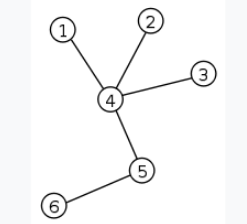
\includegraphics[height=1.5in]{../images/Tree}}

\vfill
Belief Propagation is a message passing procedure (actually dynamic programming).

\vfill
For each edge $\{i,j\}$ and possible value $\tilde{y}$ for node $i$ we define {\color{red} $Z_{j \rightarrow i}[c]$}
to be  the partition function for the subtree attached to $i$ through $j$ and
with $\hat{y}[i]$ restricted to $c$.

\vfill
The function $Z_{j \rightarrow i}$ on the possible values of node $i$ is called the {\bf message} from $j$ to $i$.

\vfill
The reverse direction message $Z_{i \rightarrow j}$ is defined similarly.

\slide{Dynamic Programming Computes the Messages}

\centerline{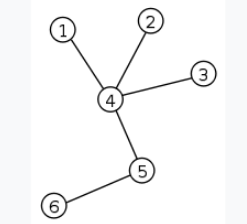
\includegraphics[height=2.0in]{../images/Tree}}

\vfill
\begin{eqnarray*}
  Z_{j\rightarrow i}[c] & = & \sum_{c'}  e^{s_n[j,c'] + s_e[j,i,c',c]}
    \left(\prod_{k \in N(j),\;k \not = i}\;Z_{k\rightarrow j}[c']\right)
\end{eqnarray*}

\slide{Loopy BP}

In a Loopy Graph we can initializing all message $Z_{i \rightarrow j}[c] = 1$ and then repeating (until convergence) the updates
\vfill
\begin{eqnarray*}
  \tilde{Z}_{j \rightarrow i}[c] & = & \frac{1}{Z_{j \rightarrow i}}\;Z_{j \rightarrow i}[c] \;\;\;\;\;Z_{j \rightarrow i} = \sum_{c} Z_{j \rightarrow i}[c] \\
  \\
  \\
  Z_{j\rightarrow i}[c] & = & \sum_{c'}  e^{s_n[j,c'] + s_e[j,i,c',c]}
    \left(\prod_{k \in N(j),\;k \not = i}\;\tilde{Z}_{k\rightarrow j}[c']\right)
\end{eqnarray*}

\anaslide{Computing Node Marginals from Messages}

\centerline{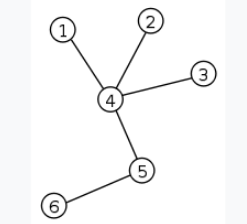
\includegraphics[height=1.5in]{../images/Tree}}

\begin{eqnarray*}
Z_i(c) & \doteq & \sum_{\hat{y}:\; \hat{y}[i] = c} \;e^{s(\hat{y})} \\
\\
& = & e^{s_i[c]} \left(\prod_{j\in N(i)} Z_{j \rightarrow i}[c]\right) \\
\\
{\color{red} P_i(c)} & = & Z_i(c)/Z,\;\;\;\;\; Z = \sum_{c}\;Z_i(c)
\end{eqnarray*}


\anaslide{Computing Edge Marginals from Messages}

\begin{eqnarray*}
Z_{i,j}(c,c') & \doteq & \sum_{\hat{y}:\; \hat{y}[i] = c,\;\hat{y}[j] = c'} \;e^{s(\hat{y})} \\
\\
& = & e^{s_n[i,c] + s_n[j,c'] +s_e[i,j,c,c']} \\
& & \prod_{k\in N(i),\;k \not = j} Z_{k \rightarrow i}[c] \\
& & \prod_{k\in N(j),\;k \not = i} Z_{k \rightarrow j}[c'] \\
\\
{\color{red} P_{i,j}(c,c')} & = & Z_{i,j}(c,c')/Z\;\;\;Z = \sum_{c,c'}\;Z_{i,j}(c,c')
\end{eqnarray*}


\slide{Summary}

We are often interested in probability distributions on structured objects such as sentence or images.

\vfill
Graphical models define softmax distributions on structured values.

\vfill
It is infeasible to enumerate all sentences or all images.

\vfill
However, pseudolikelihood provides a reasonable training algorithm and loopy BP can be used for both training time and test time
inference.

\slide{END}

}
\end{document}

\slide{An Example}

Consider an image with three superpixels $A$, $B$ and $C$ where
each superpixel is to labeled as either ``foreground'' or background.

\vfill
Suppose the unary scores are all zero.

\vfill
$$s_A(\mathrm{Foreground}) = s_A(\mathrm{Background}) = 0$$
$$s_B(\mathrm{Foreground}) = s_B(\mathrm{Background}) = 0$$
$$s_C(\mathrm{Foreground}) = s_C(\mathrm{Background}) = 0$$

\slide{The Binary Scores}


\vfill
Let $F_A$ be the proposition that $A$ is forground and similarly for $F_B$ and $F_C$.

\vfill
We can express $F_A \Rightarrow F_B$ with
$$s_{A,B}(\mathrm{Foreground},\mathrm{Background}) = -1$$
$$s_{A,B}(\mathrm{Foreground},\mathrm{Foreground}) = 1$$
$$s_{A,B}(\mathrm{Background},\mathrm{Background}) = 1$$
$$s_{A,B}(\mathrm{Background},\mathrm{Foreground}) = 1$$

\vfill
The binary scores are then given by
$F_A \Rightarrow F_B$, $F_B \Rightarrow F_C$, $F_C \Rightarrow F_A$.

\slide{The Full Configuration Score}

For any configuration $\hat{y}$ we have that $s(\hat{y})$ is the sum of the unary and binary scores.

\vfill
If none are foreground we have $s(\hat{y}) = 3$

\vfill
If one is foreground we have $s(\hat{y}) = -1 + 1+ 1 = 1$

\vfill
If two are foreground we also have $s(\hat{y}) = -1 + 1+ 1 = 1$

\vfill
If all are foreground we have $s(\hat{y}) = 3$.

\vfill
$$Z = 6*1 + 2*3 = 12\;\;\;\;P_A(\mathrm{Foregound}) = \frac{3*1 + 3}{12} = \frac{1}{2}$$



\slide{Hyper-Graphs: More General and More Concise}

A hyper-edge is a subset of nodes.

\vfill
\centerline{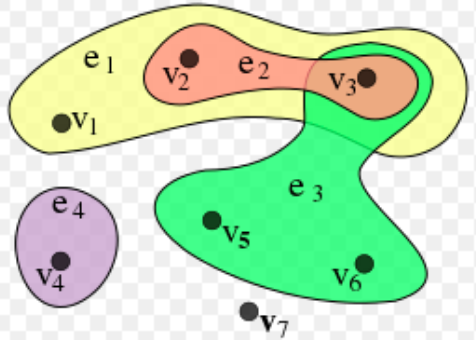
\includegraphics[height = 1.5in]{../images/HyperGraph}}


$$s(\hat{y}) = \sum_{i \in \mathrm{Nodes}}\; s_i[\hat{y}[i]]\; + \sum_{e \in \mathrm{Edges}}\;s_e[\hat{y}[e.i],\hat{y}[e.j]]$$

\vfill

$${\color{red} s(\hat{y}) = \sum_{e \in \mathrm{HyperEdges}}  \; s_e[\hat{y}[e]]}$$


\slide{Hyper-Graph Models}

We will abbreviate $s_e[\hat{y}[e]]$ as {\color{red} $s_e[\tilde{y}]$}.

\vfill
{\color{red} $\tilde{y}$ has a small number of possible values.}

\vfill
The hyper-graph model is defined by the ``tensor'' {\color{red} $s_e(\tilde{y})$}.


\slide{Back-Propagation}

The input is the image $x$ and the parameter package $\Phi$

\begin{eqnarray*}
 & \vdots & \\
s_e[\tilde{y}] & = & \ldots \\
{\cal L} & = & - \ln\; P(y\;|\;s_{\cal E}[{\cal Y}])
\end{eqnarray*}

\vfill We abbreviate $P(\hat{y}\;|\;s_{\cal E}[{\cal Y}])$ as {\color{red} $P_s(\hat{y})$} --- the distribution on $\hat{y}$ defined by the tensor $s$.
\vfill
We need to compute {\color{red} $\nabla_s -\ln P_s(y)$}, or equivalently, {\color{red} $s_e.\grad[\hat{y}[e]]$}.


